% This is LLNCS.DEM the demonstration file of
% the LaTeX macro package from Springer-Verlag
% for Lecture Notes in Computer Science,
% version 2.4 for LaTeX2e as of 16. April 2010
%
\documentclass{llncs}
%
\usepackage{makeidx}  % allows for indexgeneration
\usepackage{hyperref}
%
\begin{document}
%
\title{LHCb Topological Trigger: Approaches and Optimization}

\titlerunning{LHCb Topological Trigger}  % abbreviated title (for running head)
%                                     also used for the TOC unless
%                                     \toctitle is used
%
\author{Tatiana Likhomanenko\inst{1, 2, 3} \email{tatiana.likhomanenko@cern.ch} \and Philip Ilten\inst{5} \and Egor Khairullin\inst{1, 4} \and Alex Rogozhnikov\inst{1, 2} \and Andrey Ustyuzhanin\inst{1, 2, 3, 4} \and Michael Williams\inst{5} \email{mwill@mit.edu}}
\authorrunning{Ivar Ekeland et al.} % abbreviated author list (for running head)
%
%%%% list of authors for the TOC (use if author list has to be modified)
% \tocauthor{Ivar Ekeland, Roger Temam, Jeffrey Dean, David Grove,
% Craig Chambers, Kim B. Bruce, and Elisa Bertino}
% %
% \institute{Princeton University, Princeton NJ 08544, USA,\\
% \email{I.Ekeland@princeton.edu},\\ WWW home page:
% \texttt{http://users/\homedir iekeland/web/welcome.html}
% \and
% Universit\'{e} de Paris-Sud,
% Laboratoire d'Analyse Num\'{e}rique, B\^{a}timent 425,\\
% F-91405 Orsay Cedex, France}

\institute{ Yandex School of Data Analysis (YSDA), RU
\and
National Research University Higher School of Economics (HSE), RU
\and 
NRC "Kurchatov Institute", RU
\and 
Moscow Institute of Physics and Technology, Moscow, RU
\and 
Massachusetts Institute of Technology, US}



\maketitle              % typeset the title of the contribution

\begin{abstract}
The LHCb trigger system plays a key role in selecting events (proton-proton collisions) to store them into memory for further processing. It should choose several thousands events per second among all detected by LHCb. The main b-physics trigger algorithm (should select events with B-meson decays) used by the LHCb experiment is a so-called topological trigger. In the LHC Run 1, this trigger, which utilized a simple boosted decision tree algorithm, selected a nearly 100\% pure sample of b-hadrons with a typical efficiency of 60-70\%; its output was used in about 60\% of LHCb papers. In the paper \cite{run2_topo} we presented studies carried out to optimize the topological trigger for LHC Run 2. Trigger data have a specific structure and that is why necessary quality measure was proposed. In this paper we investigate the presense of noisy samples in data and propose several ways to reduce this noise. Anoter side of the trigger system is a real-time prediction operation: it should be very fast. In the paper \cite{run2_topo} two approaches how to speedup a prediction operation and to preserve the quality as possible were considered: bonsai boosted decision tree format (used in Run 1) and decision trees post prunning. In this paper we analyse behaviour of the cleaned up samples for these two approaches. As a result, we demonstrate that removing of noise can still improve reoptimized topological trigger on the Run 1 performance for a wide range of b-hadron decays.

\keywords{high energy physics, machine learning, LHCb trigger system}
\end{abstract}
%
% \section{Fixed-Period Problems: The Sublinear Case}
% %
% With this chapter, the preliminaries are over, and we begin the search
% for periodic solutions to Hamiltonian systems. All this will be done in
% the convex case; that is, we shall study the boundary-value problem
% \begin{eqnarray*}
%   \dot{x}&=&JH' (t,x)\\
%   x(0) &=& x(T)
% \end{eqnarray*}
% with $H(t,\cdot)$ a convex function of $x$, going to $+\infty$ when
% $\left\|x\right\| \to \infty$.

% %
% \subsection{Autonomous Systems}
% %
% In this section, we will consider the case when the Hamiltonian $H(x)$
% is autonomous. For the sake of simplicity, we shall also assume that it
% is $C^{1}$.

% We shall first consider the question of nontriviality, within the
% general framework of
% $\left(A_{\infty},B_{\infty}\right)$-subquadratic Hamiltonians. In
% the second subsection, we shall look into the special case when $H$ is
% $\left(0,b_{\infty}\right)$-subquadratic,
% and we shall try to derive additional information.
% %
% \subsubsection{The General Case: Nontriviality.}
% %
% We assume that $H$ is
% $\left(A_{\infty},B_{\infty}\right)$-sub\-qua\-dra\-tic at infinity,
% for some constant symmetric matrices $A_{\infty}$ and $B_{\infty}$,
% with $B_{\infty}-A_{\infty}$ positive definite. Set:
% \begin{eqnarray}
% \gamma :&=&{\rm smallest\ eigenvalue\ of}\ \ B_{\infty} - A_{\infty} \\
%   \lambda : &=& {\rm largest\ negative\ eigenvalue\ of}\ \
%   J \frac{d}{dt} +A_{\infty}\ .
% \end{eqnarray}

% Theorem~\ref{ghou:pre} tells us that if $\lambda +\gamma < 0$, the
% boundary-value problem:
% \begin{equation}
% \begin{array}{rcl}
%   \dot{x}&=&JH' (x)\\
%   x(0)&=&x (T)
% \end{array}
% \end{equation}
% has at least one solution
% $\overline{x}$, which is found by minimizing the dual
% action functional:
% \begin{equation}
%   \psi (u) = \int_{o}^{T} \left[\frac{1}{2}
%   \left(\Lambda_{o}^{-1} u,u\right) + N^{\ast} (-u)\right] dt
% \end{equation}
% on the range of $\Lambda$, which is a subspace $R (\Lambda)_{L}^{2}$
% with finite codimension. Here
% \begin{equation}
%   N(x) := H(x) - \frac{1}{2} \left(A_{\infty} x,x\right)
% \end{equation}
% is a convex function, and
% \begin{equation}
%   N(x) \le \frac{1}{2}
%   \left(\left(B_{\infty} - A_{\infty}\right) x,x\right)
%   + c\ \ \ \forall x\ .
% \end{equation}

% %
% \begin{proposition}
% Assume $H'(0)=0$ and $ H(0)=0$. Set:
% \begin{equation}
%   \delta := \liminf_{x\to 0} 2 N (x) \left\|x\right\|^{-2}\ .
%   \label{eq:one}
% \end{equation}

% If $\gamma < - \lambda < \delta$,
% the solution $\overline{u}$ is non-zero:
% \begin{equation}
%   \overline{x} (t) \ne 0\ \ \ \forall t\ .
% \end{equation}
% \end{proposition}
% %
% \begin{proof}
% Condition (\ref{eq:one}) means that, for every
% $\delta ' > \delta$, there is some $\varepsilon > 0$ such that
% \begin{equation}
%   \left\|x\right\| \le \varepsilon \Rightarrow N (x) \le
%   \frac{\delta '}{2} \left\|x\right\|^{2}\ .
% \end{equation}

% It is an exercise in convex analysis, into which we shall not go, to
% show that this implies that there is an $\eta > 0$ such that
% \begin{equation}
%   f\left\|x\right\| \le \eta
%   \Rightarrow N^{\ast} (y) \le \frac{1}{2\delta '}
%   \left\|y\right\|^{2}\ .
%   \label{eq:two}
% \end{equation}

% \begin{figure}
% \vspace{2.5cm}
% \caption{This is the caption of the figure displaying a white eagle and
% a white horse on a snow field}
% \end{figure}

% Since $u_{1}$ is a smooth function, we will have
% $\left\|hu_{1}\right\|_\infty \le \eta$
% for $h$ small enough, and inequality (\ref{eq:two}) will hold,
% yielding thereby:
% \begin{equation}
%   \psi (hu_{1}) \le \frac{h^{2}}{2}
%   \frac{1}{\lambda} \left\|u_{1} \right\|_{2}^{2} + \frac{h^{2}}{2}
%   \frac{1}{\delta '} \left\|u_{1}\right\|^{2}\ .
% \end{equation}

% If we choose $\delta '$ close enough to $\delta$, the quantity
% $\left(\frac{1}{\lambda} + \frac{1}{\delta '}\right)$
% will be negative, and we end up with
% \begin{equation}
%   \psi (hu_{1}) < 0\ \ \ \ \ {\rm for}\ \ h\ne 0\ \ {\rm small}\ .
% \end{equation}

% On the other hand, we check directly that $\psi (0) = 0$. This shows
% that 0 cannot be a minimizer of $\psi$, not even a local one.
% So $\overline{u} \ne 0$ and
% $\overline{u} \ne \Lambda_{o}^{-1} (0) = 0$. \qed
% \end{proof}
% %
% \begin{corollary}
% Assume $H$ is $C^{2}$ and
% $\left(a_{\infty},b_{\infty}\right)$-subquadratic at infinity. Let
% $\xi_{1},\allowbreak\dots,\allowbreak\xi_{N}$  be the
% equilibria, that is, the solutions of $H' (\xi ) = 0$.
% Denote by $\omega_{k}$
% the smallest eigenvalue of $H'' \left(\xi_{k}\right)$, and set:
% \begin{equation}
%   \omega : = {\rm Min\,} \left\{\omega_{1},\dots,\omega_{k}\right\}\ .
% \end{equation}
% If:
% \begin{equation}
%   \frac{T}{2\pi} b_{\infty} <
%   - E \left[- \frac{T}{2\pi}a_{\infty}\right] <
%   \frac{T}{2\pi}\omega
%   \label{eq:three}
% \end{equation}
% then minimization of $\psi$ yields a non-constant $T$-periodic solution
% $\overline{x}$.
% \end{corollary}
% %

% We recall once more that by the integer part $E [\alpha ]$ of
% $\alpha \in \bbbr$, we mean the $a\in \bbbz$
% such that $a< \alpha \le a+1$. For instance,
% if we take $a_{\infty} = 0$, Corollary 2 tells
% us that $\overline{x}$ exists and is
% non-constant provided that:

% \begin{equation}
%   \frac{T}{2\pi} b_{\infty} < 1 < \frac{T}{2\pi}
% \end{equation}
% or
% \begin{equation}
%   T\in \left(\frac{2\pi}{\omega},\frac{2\pi}{b_{\infty}}\right)\ .
%   \label{eq:four}
% \end{equation}

% %
% \begin{proof}
% The spectrum of $\Lambda$ is $\frac{2\pi}{T} \bbbz +a_{\infty}$. The
% largest negative eigenvalue $\lambda$ is given by
% $\frac{2\pi}{T}k_{o} +a_{\infty}$,
% where
% \begin{equation}
%   \frac{2\pi}{T}k_{o} + a_{\infty} < 0
%   \le \frac{2\pi}{T} (k_{o} +1) + a_{\infty}\ .
% \end{equation}
% Hence:
% \begin{equation}
%   k_{o} = E \left[- \frac{T}{2\pi} a_{\infty}\right] \ .
% \end{equation}

% The condition $\gamma < -\lambda < \delta$ now becomes:
% \begin{equation}
%   b_{\infty} - a_{\infty} <
%   - \frac{2\pi}{T} k_{o} -a_{\infty} < \omega -a_{\infty}
% \end{equation}
% which is precisely condition (\ref{eq:three}).\qed
% \end{proof}
% %

% \begin{lemma}
% Assume that $H$ is $C^{2}$ on $\bbbr^{2n} \setminus \{ 0\}$ and
% that $H'' (x)$ is non-de\-gen\-er\-ate for any $x\ne 0$. Then any local
% minimizer $\widetilde{x}$ of $\psi$ has minimal period $T$.
% \end{lemma}
% %
% \begin{proof}
% We know that $\widetilde{x}$, or
% $\widetilde{x} + \xi$ for some constant $\xi
% \in \bbbr^{2n}$, is a $T$-periodic solution of the Hamiltonian system:
% \begin{equation}
%   \dot{x} = JH' (x)\ .
% \end{equation}

% There is no loss of generality in taking $\xi = 0$. So
% $\psi (x) \ge \psi (\widetilde{x} )$
% for all $\widetilde{x}$ in some neighbourhood of $x$ in
% $W^{1,2} \left(\bbbr / T\bbbz ; \bbbr^{2n}\right)$.

% But this index is precisely the index
% $i_{T} (\widetilde{x} )$ of the $T$-periodic
% solution $\widetilde{x}$ over the interval
% $(0,T)$, as defined in Sect.~2.6. So
% \begin{equation}
%   i_{T} (\widetilde{x} ) = 0\ .
%   \label{eq:five}
% \end{equation}

% Now if $\widetilde{x}$ has a lower period, $T/k$ say,
% we would have, by Corollary 31:
% \begin{equation}
%   i_{T} (\widetilde{x} ) =
%   i_{kT/k}(\widetilde{x} ) \ge
%   ki_{T/k} (\widetilde{x} ) + k-1 \ge k-1 \ge 1\ .
% \end{equation}

% This would contradict (\ref{eq:five}), and thus cannot happen.\qed
% \end{proof}
% %
% \paragraph{Notes and Comments.}
% The results in this section are a
% refined version of \cite{clar:eke};
% the minimality result of Proposition
% 14 was the first of its kind.

% To understand the nontriviality conditions, such as the one in formula
% (\ref{eq:four}), one may think of a one-parameter family
% $x_{T}$, $T\in \left(2\pi\omega^{-1}, 2\pi b_{\infty}^{-1}\right)$
% of periodic solutions, $x_{T} (0) = x_{T} (T)$,
% with $x_{T}$ going away to infinity when $T\to 2\pi \omega^{-1}$,
% which is the period of the linearized system at 0.

% \begin{table}
% \caption{This is the example table taken out of {\it The
% \TeX{}book,} p.\,246}
% \begin{center}
% \begin{tabular}{r@{\quad}rl}
% \hline
% \multicolumn{1}{l}{\rule{0pt}{12pt}
%                    Year}&\multicolumn{2}{l}{World population}\\[2pt]
% \hline\rule{0pt}{12pt}
% 8000 B.C.  &     5,000,000& \\
%   50 A.D.  &   200,000,000& \\
% 1650 A.D.  &   500,000,000& \\
% 1945 A.D.  & 2,300,000,000& \\
% 1980 A.D.  & 4,400,000,000& \\[2pt]
% \hline
% \end{tabular}
% \end{center}
% \end{table}
% %
% \begin{theorem} [Ghoussoub-Preiss]\label{ghou:pre}
% Assume $H(t,x)$ is
% $(0,\varepsilon )$-subquadratic at
% infinity for all $\varepsilon > 0$, and $T$-periodic in $t$
% \begin{equation}
%   H (t,\cdot )\ \ \ \ \ {\rm is\ convex}\ \ \forall t
% \end{equation}
% \begin{equation}
%   H (\cdot ,x)\ \ \ \ \ {\rm is}\ \ T{\rm -periodic}\ \ \forall x
% \end{equation}
% \begin{equation}
%   H (t,x)\ge n\left(\left\|x\right\|\right)\ \ \ \ \
%   {\rm with}\ \ n (s)s^{-1}\to \infty\ \ {\rm as}\ \ s\to \infty
% \end{equation}
% \begin{equation}
%   \forall \varepsilon > 0\ ,\ \ \ \exists c\ :\
%   H(t,x) \le \frac{\varepsilon}{2}\left\|x\right\|^{2} + c\ .
% \end{equation}

% Assume also that $H$ is $C^{2}$, and $H'' (t,x)$ is positive definite
% everywhere. Then there is a sequence $x_{k}$, $k\in \bbbn$, of
% $kT$-periodic solutions of the system
% \begin{equation}
%   \dot{x} = JH' (t,x)
% \end{equation}
% such that, for every $k\in \bbbn$, there is some $p_{o}\in\bbbn$ with:
% \begin{equation}
%   p\ge p_{o}\Rightarrow x_{pk} \ne x_{k}\ .
% \end{equation}
% \qed
% \end{theorem}
% %
% \begin{example} [{{\rm External forcing}}]
% Consider the system:
% \begin{equation}
%   \dot{x} = JH' (x) + f(t)
% \end{equation}
% where the Hamiltonian $H$ is
% $\left(0,b_{\infty}\right)$-subquadratic, and the
% forcing term is a distribution on the circle:
% \begin{equation}
%   f = \frac{d}{dt} F + f_{o}\ \ \ \ \
%   {\rm with}\ \ F\in L^{2} \left(\bbbr / T\bbbz; \bbbr^{2n}\right)\ ,
% \end{equation}
% where $f_{o} : = T^{-1}\int_{o}^{T} f (t) dt$. For instance,
% \begin{equation}
%   f (t) = \sum_{k\in \bbbn} \delta_{k} \xi\ ,
% \end{equation}
% where $\delta_{k}$ is the Dirac mass at $t= k$ and
% $\xi \in \bbbr^{2n}$ is a
% constant, fits the prescription. This means that the system
% $\dot{x} = JH' (x)$ is being excited by a
% series of identical shocks at interval $T$.
% \end{example}
% %
% \begin{definition}
% Let $A_{\infty} (t)$ and $B_{\infty} (t)$ be symmetric
% operators in $\bbbr^{2n}$, depending continuously on
% $t\in [0,T]$, such that
% $A_{\infty} (t) \le B_{\infty} (t)$ for all $t$.

% A Borelian function
% $H: [0,T]\times \bbbr^{2n} \to \bbbr$
% is called
% $\left(A_{\infty} ,B_{\infty}\right)$-{\it subquadratic at infinity}
% if there exists a function $N(t,x)$ such that:
% \begin{equation}
%   H (t,x) = \frac{1}{2} \left(A_{\infty} (t) x,x\right) + N(t,x)
% \end{equation}
% \begin{equation}
%   \forall t\ ,\ \ \ N(t,x)\ \ \ \ \
%   {\rm is\ convex\ with\  respect\  to}\ \ x
% \end{equation}
% \begin{equation}
%   N(t,x) \ge n\left(\left\|x\right\|\right)\ \ \ \ \
%   {\rm with}\ \ n(s)s^{-1}\to +\infty\ \ {\rm as}\ \ s\to +\infty
% \end{equation}
% \begin{equation}
%   \exists c\in \bbbr\ :\ \ \ H (t,x) \le
%   \frac{1}{2} \left(B_{\infty} (t) x,x\right) + c\ \ \ \forall x\ .
% \end{equation}

% If $A_{\infty} (t) = a_{\infty} I$ and
% $B_{\infty} (t) = b_{\infty} I$, with
% $a_{\infty} \le b_{\infty} \in \bbbr$,
% we shall say that $H$ is
% $\left(a_{\infty},b_{\infty}\right)$-subquadratic
% at infinity. As an example, the function
% $\left\|x\right\|^{\alpha}$, with
% $1\le \alpha < 2$, is $(0,\varepsilon )$-subquadratic at infinity
% for every $\varepsilon > 0$. Similarly, the Hamiltonian
% \begin{equation}
% H (t,x) = \frac{1}{2} k \left\|k\right\|^{2} +\left\|x\right\|^{\alpha}
% \end{equation}
% is $(k,k+\varepsilon )$-subquadratic for every $\varepsilon > 0$.
% Note that, if $k<0$, it is not convex.
% \end{definition}
% %


\section{Introduction}
The LHCb detector \cite{detector} is designed for studying beauty and charm (heavy flavour) hadrons produced in proton-proton collisions at the Large Hadron Collider (LHC) at CERN.
At LHCb data were collected with the rate 40 MHz in Run 1 ($40*10^6$ proton-proton collisions, called events, per second). This amount cannot be store into memory. A trigger system hardware part, called Level-0 (L0), reduced the visible bunch crossing rate to 1 MHz at which the detector could be read out. Further, a flexible software High-Level Trigger (HLT) applied a range of more advanced selections that reduce the rate to about 5 kHz ($5 * 10^3$ events per second) for offline storage and processing. This configuration allowed LHCb to record the largest beauty and charm hadron samples at a very high signal purity. The performance of the Run 1 trigger is described in detail in \cite{run1_1}, \cite{run1_2}.

In Run 1 it was shown that complex, multivariate trigger selections were possible. The HLT processes few enough events that it is possible to perform the reconstruction of a collision (to reconstruct tracks, vertices, a topology, physical characteristics). There are many HLT lines dedicated to triggering on various types of events. The majority of analyses using b-hadrons at LHCb made use of the topological n-body trigger \cite{run1_topo}. Most n-body hadronic B decays $(n \geq 3)$ are only triggered on efficiently in LHCb by these lines. The topological n-body trigger is an inclusive trigger which combines successive 2,3 and 4-body track combinations. A novel boosted decision trees (BDT) multivariate selection \cite{bbdt} was used in Run 1. 

In the \cite{run2_topo} we studied upgrading of the topological trigger: a new scheme of the trigger processing, which includes a more widespread usage of machine learning, was proposed; the appropriate quality measure was considered (receiver operating characteristic, ROC, computed for events for all B decays). However, obtained algorithms cannot be used in real-time trigger data processing. That is why, in the paper \cite{run2_topo} we compared two approaches how to speedup a prediction operation: bonsai boosted decision tree format \cite{bbdt} and decision trees post prunning. 

In the previous analysis \cite{run2_topo} simulated data for various B decays were used as signal-like samples and real data from the collider without any physics were used as background-like samples. In this paper we present studies connected with the fact that simulated samples contain noisy data. We propose several ways how to clean up the samples and analyse the quality of the two speedup approaches in this case. As a result, we demonstrate that removing of noise can still improve the reoptimized topological trigger on the Run 1 performance for a wide range of b-hadron decays.

\section{Motivation}
Data for the trigger system have a specific structure: each event consists of the several reconstructed secondary vertices; a set of all secondary vertices for all B decays are the training sample. After training an event will pass the trigger if at least one its secondary vertex will pass the trigger (passing the trigger means that a prediction for a sample is greater than some fixed threshold; a threshold is chosen in a way that the false positive rate value provides the trigger rate). And we are interested in the greatest true positive rate for each B-decay mode. 

As background-like data we use real data from the collider without any physics (that is why chosing the trigger rate will be equivalent to chosing the false posive rate). It means that all reconstructed secondary vertices for each event in the background-like data don't contain any interesting decays. As signal-like data we use the proton-proton collisions simulated for each mode of B-decays. For these data we really know that at least in one secondary vertex necessary decay happened. But it doesn't guaratee that all secondary vertices contain interesting B-decays.

Each event can contain up to 40 secondary vertices. For the signal-like data one of these is a truly signal-like sample, but others can be noise.

\section{Noise clean up approaches}

\section{Speedup approaches with cleaned up samples}

\section{Conclusion}

In the HLT1 during Run 1, the so-called  "1 track" line was used because there was not sufficient CPU time for combinatorics and because the tracking transverse momentum threshold was too high for an secondary vertex (SV) based approach to be efficient. In Run 2, the HLT1 tracking transverse momentum threshold will be the same as was used in the HLT2 for Run 1.  This makes it possible to use, along with a "1 track" line, a "2 body SV" line. Thus, we consider a new HLT scheme (figure~\ref{scheme}). The combination of displacement from the primary vertex (PV) and high transverse momentum are the main characteristics of interesting decays. The HLT "1-track" line is looking for either one super high transverse momentum or high displacement track. The HLT "2 body SV" line uses a multivariate analysis to look for two tracks that form a vertex. The HLT topological line is improved using a more powerful multivariate analysis. It uses fully reconstructed events to look for 2, 3, and 4 tracks making a vertex.

The analysis was conducted on the following data: signal samples are simulated 13-TeV B-decays of various topologies, while the background sample is generic Pythia 13-TeV proton-proton collisions.

\begin{figure}[h]
\includegraphics[width=16pc]{images/scheme.pdf}\hspace{2pc}%
\begin{minipage}[b]{20pc}\caption{\label{scheme} HLT Run 2 scheme. HLT1 consists of two lines: the "1-track" and "2 body SV", with corresponding output rates 100 kHz and 50 kHz. If an event passes at least one of these two lines, then it is triggered by the topological line with output rate 2-4 kHz.}
\end{minipage}
\end{figure}

\section{Noise clean up approaches}
Each event is represented as set of secondary vertices. These secondary vertices are the input data to the classifier.  The event is triggered if at least one secondary vertex passes the classifier selection. A trigger's output rate is limited. This restriction is equivalent to a restriction on the background events efficiency (FPR). For example, for an output rate of 2 kHz, then FPR is 0.2\%. This can be shown using ROC curves from the classifier, which are plotted for test events (figure~\ref{roc}).

All classifiers were trained on one half of the data and were tested on the other half. For the HLT "1-track" and "2 body SV" lines, all signal modes were used, while for the HLT topological line six specific modes were used in training.  All algorithms were tested on all available signal modes.

\begin{figure}[h]
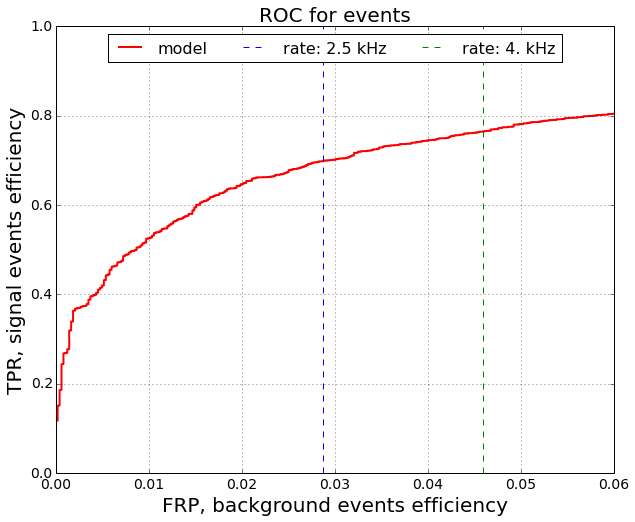
\includegraphics[width=22pc]{images/roc_events.pdf}\hspace{2pc}%
\begin{minipage}[b]{14pc}\caption{\label{roc} Trigger events ROC curve. An output rate of 2.5 kHz corresponds to an FPR of 0.25\%, 4 kHz~--- 0.4\%. Thus to find the signal efficiency for a 2.5 kHz output rate, we take 0.25\% background efficiency and find the point on the ROC curve that corresponds to this FPR.}
\end{minipage}
\end{figure}

\subsection{HLT "1-track" line}
Preselections and variables for the HLT "1-track" line are listed in table~\ref{hlt1sel}. Only two variables are used in this line. To optimize the signal efficiency and find an optimal decision boundary,  multivariate analysis is used. Distributions of signal and background are shown in figure~\ref{hlt1}. The MatrixNet\cite{mn_paper} algorithm (figure~\ref{hlt1mn}), logistic regression (figure~\ref{hlt1log}) and neural networks (figure~\ref{hlt1nn}) were trained to find the decision boundaries. From experiments, MatrixNet decision boundary is found to be the best, but for online processing a more simple decision rule fits: a hyperbolic function can be used as the decision boundary. Efficiencies comparison of different algorithms for B-modes is shown in figure~\ref{hlt1_res}.


\begin{figure}[h]
\begin{minipage}{18pc}
\includegraphics[width=18pc]{images/track-db}
\caption{\label{hlt1} Track data scatters, described in two-dimensional space.}
\end{minipage}\hspace{2pc}%
\begin{minipage}{18pc}
\includegraphics[width=18pc]{images/log-track-db}
\caption{\label{hlt1log} Decision boundary for logistic regression.}
\end{minipage} 
\begin{minipage}{18pc}\vspace{1pc}%
\includegraphics[width=18pc]{images/mn-track-db}
\caption{\label{hlt1mn} Decision boundary for MatrixNet algorithm.}
\end{minipage}\hspace{2pc}%
\begin{minipage}{18pc}\vspace{1pc}%
\includegraphics[width=18pc]{images/nn-track-db}
\caption{\label{hlt1nn} Decision boundary for neural networks.}
\end{minipage} 
\end{figure}


\begin{center}
\begin{table}[h]
\centering
    \caption{\label{hlt1sel} HLT "1-track" line description.}
    %\footnotesize\rm
    \centering
    \begin{tabular}{@{}*{7}{l}}
    \br
    Track preselections: & \\
    
    \verb  & $PT > 500$ MeV\\
    \verb  & $IP_{\chi^2} > 4$\\
    \verb  & $track_{\chi^2}/ndof < 3$\\
    \br
    Analysis variables: & $PT$, $IP_{\chi^2}$ \\
    \br
    Output rate: & 100 kHz\\
    \br
    \end{tabular}
\end{table}
\end{center}


\subsection{HLT "2 body SV" line}
Preselections and variables for the HLT "2 body SV" line are listed in table \ref{hlt1svsel}. The line looks for two tracks that form a vertex. In this case, the MatrixNet algorithm is used and several studies were conducted. Firstly, the possibility to remove the corrected mass cut ($mcor<10$) and to remove the corrected mass as variable from classifier's input was investigated.  The impact on the performance is negligible.  These removals were done to reduce systematic uncertainties and to help in exotic searches. Secondly, to minimize the set of variables used in trigger, a selection was conducted among the scalar sum, vector sum, and minimum of the transverse momenta. The results obtained (efficiencies comparison) are shown in figure \ref{hlt12_res}.

\begin{figure}[h]
\begin{minipage}{18pc}
\includegraphics[width=18pc]{images/track.pdf}
\caption{\label{hlt1_res} Efficiencies comparison for MatrixNet (MN), neural networks (NN) and logistic regression. 50 kHz and 100 kHz output rates are considered. \\ \\ \\ }
\end{minipage}\hspace{2pc}%
\begin{minipage}{18pc}
\includegraphics[width=18pc]{images/hlt1-2body.pdf}
\caption{\label{hlt12_res} Efficiencies comparison for MatrixNet: with corrected mass, without it (MN), with the scalar sum of transverse momentum (sum $pt$, without min and vector $pt$). These models were `converted' to BBDT format and compared. The output rate is set to 50~kHz.}
\end{minipage} 
\end{figure}


\begin{table}[h]
%\centering
\begin{minipage}{.48\textwidth}
  %\centering
    \caption{\label{hlt1svsel} HLT "2 body SV" line description.}
    %\footnotesize\rm
    \centering
    \begin{tabular}{@{}*{2}{l}}
    \br
    Track preselections: \hspace{-1cm} & \\
    
    \verb  & $PT > 500$ MeV\\
    \verb  & $IP_{\chi^2} > 4$\\
    \verb  & $track_{\chi^2}/ndof < 2.5$\\
    \br
    SV preselections: \hspace{-1cm} & \\
    
    \verb  & $PT > 2$ GeV\\
    \verb  & $vertex_{\chi^2} < 10$ \\
    \verb  & $1 < mcor$ GeV \\
    \verb  & $2 < \eta < 5$ (PV to SV) \\
    \br
    Analysis variables: \hspace{-1cm} & \\
    \verb  & sum $PT$, $vertex_{\chi^2}$, $FD_{\chi_2}$,  \\
    \verb  & $N$(tracks with $IP_{\chi^2} < 16$) \\ 
     \verb  & \\ 
      \verb  & \\ 
    \br
    Output rate: \hspace{-1cm} & 50 kHz\\
    \br
    \end{tabular}
  \end{minipage}
%\centering  
%\hspace{0.5pc}
\begin{minipage}{.45\textwidth}
  \caption{\label{hlt2sel} HLT topological line description.}
%\footnotesize\rm
   % \centering
    \begin{tabular}{@{}*{2}{l}}
    \br
    Track preselections: \hspace{-1cm} & \\
    
    \verb  & $PT > 200$ MeV\\
    \verb  & $IP_{\chi^2} > 4$\\
    \verb  & $track_{\chi^2}/ndof < 2.5$\\
    \br
    SV preselections: \hspace{-1cm} & \\
    
    \verb  & $vertex_{\chi^2} < 10$ \\
    \verb  & $1 < mcor < 10$ GeV \\
    \verb  & $2 < \eta < 5$ (PV to SV) \\
    \verb  & $N$(tracks with $IP_{\chi^2} < 16) < 2$\\
    \br
    Analysis variables: \hspace{-1cm} & \\
    \verb  & n, mcor, sum $PT$, $vertex_{\chi^2}$, \\
    \verb  & $\eta$, $FD_{\chi_2}$, min $PT$, \\
    \verb  & $IP_{\chi^2}$, $N$(tracks), \\
    \verb  & $N$(tracks with $IP_{\chi^2} < 16$) \\ 
    \br
    Output rate: \hspace{-1cm} & 2-4 kHz\\
    \br
    \end{tabular}
  \end{minipage}
\end{table}

\subsection{HLT topological line}
The HLT2 topological lines are designed to trigger efficiently on any B decay with at least 2 charged children. It is designed to handle the possible omission of child particles.  To save CPU time in the HLT2 reconstruction, only tracks with transverse momentum $PT > 200$ MeV are reconstructed. To reduce the background rate due to ghosts, all tracks are required to have a $track_{\chi^2}/ndof$ value less than 2.5. To reduce the background rate due to prompt particles, all tracks are required to have an impact parameter $\chi^2$ value greater than 4. Due to the inclusive nature of the HLT2 topological lines, this does not mean that all of the B daughters need to satisfy these criteria. The trigger is designed to allow for the omission of one or more daughters when forming the trigger candidate. The previous topological line for Run 1 is described in \cite{topo_2}. 

In the HLT topological line used in Run 1, a simple boosted decision tree was used \cite{topo_2} to define interesting secondary vertices. For Run 2, the algorithm is reoptimized.  Current preselections and training variables are listed in table \ref{hlt2sel}. The output rate is one of the signal efficiencies factor.  The efficiency dependence on the output rate is shown in figure \ref{hlt2_out}. Thus, several modes, including two training ones, significantly depend on the output rate. 

\begin{figure}[h]
\begin{minipage}{18pc}
\includegraphics[width=18pc]{images/rates_small.pdf}
\end{minipage}\hspace{2pc}%
\begin{minipage}{18pc}
\vspace{+0.4cm}
\includegraphics[width=18pc]{images/rates.pdf}
\end{minipage} 
\caption{\label{hlt2_out} Signal efficiencies for training modes (left) and other available modes (right) for different output rates.}
\end{figure}

Different boosted decision trees were trained (figure~\ref{hlt2_blend}). Also some hierarchical algorithm was conducted, a so-called `blend'. Training data was divided into two parts. On the first part three MatrixNet classifiers were trained, which use only 2, 3 or 4 body decays as inputs. Next, the second part was predicted by the corresponding n-body classifiers. These predictions are considered as new additional input variables. The resulting MatrixNet was trained on this second part using basic variables and these additional ones. This hierarchical algorithm gives an improvement for several training modes.

\begin{figure}[h]
\begin{minipage}{18pc}
\vspace{1cm}
\includegraphics[width=18pc]{images/blend.pdf}
\end{minipage}\hspace{2pc}%
\begin{minipage}{18pc}
\vspace{-0.3cm}
\includegraphics[width=18pc]{images/hlt_mns.pdf}
\end{minipage} 
\caption{\label{hlt2_blend} Comparison of different algorithms: MatrixNet (MN), MatrixNet with SV weights (MN reweight), scikit-learn AdaBoost implementation (AdaBoost), TMVA AdaBoost implementation (TMVA) and some hierarchical algorithm (blend).}
\end{figure}

Based on these studies, the MatrixNet (MN) model was chosen. Its efficiency was compared with the Run 1 algorithm. For these six training modes, we obtain significant relative improvement: 15-60\% for 2.5 kHz output rate and 50-80\% for 4 kHz (table~\ref{hlt2res}).

\begin{center}
\begin{table}[h]
\caption{\label{hlt2res} Ratio of Run-2 over Run-1 for HLT2/HLT1 efficiencies. 
Note that the denominator is reconstructible with $PT(B)>2$~GeV, $\tau(B)>0.2$~ps.}
%\footnotesize\rm
\centering
\begin{tabular}{@{}*{7}{l}{l}}
\br
mode & 2.5 kHz & 4. kHz \\
\mr
    $B^0\to K^*[K^+\pi^-]\mu^+\mu^-$ & 1.64 & 1.72   \\ 
    $B^+\to \pi^+K^-K^+$ & 1.59 & 1.65 \\ 
    $B^0_s\to D_s^-[K^+K^-\pi^-]\mu^+\nu_\mu$ & 1.14 & 1.47 \\ 
    $B^0_s\to \psi(1S)[\mu^+\mu^-]K^+K^-\pi^+\pi^-$ & 1.62 & 1.71 \\ 
    $B^0_s\to D_s^-[K^+K^-\pi^-]\pi^+$ & 1.46 & 1.52 \\ 
    $B^0\to D^+[K^-\pi^+\pi^+]D^-[K^+\pi^-\pi^-]$ & 1.40 & 1.86  \\
\br
\end{tabular}
\end{table}
\end{center}


\section{Online processing}
Boosted decision trees are not appropriate for online processing events in triggers due to their low speed. Two approaches exist to overcome this restriction.   One is the so-called bonsai boosted decision format\cite{bbdt} (shortly BBDT).  Since it is a type of BDT, MatrixNet can be converted into this format. The second approach is post-prunning: the basic MatrixNet classifier includes several thousand trees, and the post-prunning procedure reduces this amount to a few hundred. This results in significant speedup of the prediction rate.  Both methods reduce MatrixNet signal efficiencies.  In case of the BBDT, we are also limited in the size of BBDT lookup table in RAM.  Different BBDT versions for MatrixNet were tried and compared to post-prunning to find the optimal solution for online processing (see figure~\ref{hlt2_prun}).
\begin{figure}[h]
\begin{minipage}{18pc}
\includegraphics[width=18pc]{images/prun-base.pdf}
\end{minipage}\hspace{2pc}%
\begin{minipage}{18pc}
\vspace{0.3cm}
\includegraphics[width=18pc]{images/prun.pdf}
\end{minipage} 
\caption{\label{hlt2_prun} Comparison of basic MatrixNet (base MN), BBDT format (BBDT MN) and post-prunned MatrixNet (Prunned MN)}
\end{figure}

Interestingly, the preference between the BBDT and post-prunning depends on the chosen output rate. It is clear in figure~ \ref{hlt2_prunroc}, that the ROCs order depends on the background efficiency (or the output rate). Another study for Run 2 triggers is connected to a timing comparison of BBDT and post-prunning, which is in progress at this moment.

\begin{figure}[h]
\includegraphics[width=16pc]{images/hlt2_prunroc.pdf}\hspace{2pc}%
\begin{minipage}[b]{22pc}\caption{\label{hlt2_prunroc} The best model among BBDT and post-prunning depends on background efficiency.}
\end{minipage}
\end{figure}


\section{Conclusion}
The LHCb topological trigger was successfully reoptimized for Run 2: 15-60\% efficiency improvement was obtained for 2.5 kHz output rate and 50-80\% for 4 kHz.  The presented HLT scheme will be applied in Run 2.

\paragraph{Notes and Comments.}
The part of the topological trigger analysis connected with the machine learning studies and presented in this paper and \cite{run2_topo} are open source and can be found on the github (\url{https://github.com/tata-antares/LHCb-topo-trigger}).
%
% ---- Bibliography ----
%
\begin{thebibliography}{5}
%
\bibitem{run2_topo} Likhomanenko T., Ilten P., Khairullin E., Rogozhnikov A., Ustyuzhanin A., Williams M.: 
LHCb Topological Trigger Reoptimization. Journal of Physics: Conference Series 664 (2015) 082025 [arXiv:1510.00572]

\bibitem{detector}  A. A. Alves Jr. et al.: The LHCb Detector at the LHC, JINST 3, S08005 (2008)

\bibitem{run1_1} Aaij, R., {\em et al.} [LHCb Trigger Group]: 
The LHCb trigger and its performance.
JINST {\bf 8} P04022 (2013) [arXiv:1211.3055]

\bibitem{run1_2} Aaij R. et al.: 
Performance of the LHCb High Level Trigger in 2012, J. Phys., Conf. Ser. 513, 012001 (2014).

\bibitem{run1_topo} Gligorov V., Thomas C., Williams M.: 
The HLT inclusive B triggers. Technical Report
LHCb-PUB-2011-016. CERN-LHCb-PUB-2011-016. LHCb-INT-2011-030, CERN, Geneva, Sep 2011. LHCb-INT-2011-030.

\bibitem{bbdt} Gligorov V., Williams, M.:
Efficient, reliable and fast high-level triggering using a bonsai boosted decision tree.
JINST {\bf 8}, P02013 (2013) [arXiv:1210.6861]

\bibitem{mn_paper} Gulin, A., Kuralenok, I., Pavlov, D.:
Winning the transfer learning track of Yahoo's Learning to Rank Challenge with YetiRank.
JMLR: Workshop and Conference Proceedings 14 (2011) 63 (Yandex MatrixNet).

% \bibitem {clar:eke}
% Clarke, F., Ekeland, I.:
% Nonlinear oscillations and
% boundary-value problems for Hamiltonian systems.
% Arch. Rat. Mech. Anal. 78, 315--333 (1982)

% \bibitem {clar:eke:2}
% Clarke, F., Ekeland, I.:
% Solutions p\'{e}riodiques, du
% p\'{e}riode donn\'{e}e, des \'{e}quations hamiltoniennes.
% Note CRAS Paris 287, 1013--1015 (1978)

% \bibitem {mich:tar}
% Michalek, R., Tarantello, G.:
% Subharmonic solutions with prescribed minimal
% period for nonautonomous Hamiltonian systems.
% J. Diff. Eq. 72, 28--55 (1988)

% \bibitem {tar}
% Tarantello, G.:
% Subharmonic solutions for Hamiltonian
% systems via a $\bbbz_{p}$ pseudoindex theory.
% Annali di Matematica Pura (to appear)

% \bibitem {rab}
% Rabinowitz, P.:
% On subharmonic solutions of a Hamiltonian system.
% Comm. Pure Appl. Math. 33, 609--633 (1980)

\end{thebibliography}

\end{document}
